\subsection{Parametric methods}

We load the package with the following command.


\begin{Schunk}
\begin{Sinput}
R> library("termstrc")
\end{Sinput}
\end{Schunk}

In the next steps we load the data set \proglang{govbonds} and explore its structure.

\begin{Schunk}
\begin{Sinput}
R> data(govbonds)
R> summary(govbonds)
\end{Sinput}
\begin{Soutput}
        Length Class  Mode
GERMANY 8      -none- list
AUSTRIA 8      -none- list
BELGIUM 8      -none- list
FINLAND 8      -none- list
FRANCE  8      -none- list
SPAIN   8      -none- list
\end{Soutput}
\end{Schunk}

It includes data for government bonds of eight European countries. The bonds are classified by their \emph{International Securities Identifying Number (ISIN)}, and all the necessary information on the future cash flows is given.

\begin{Schunk}
\begin{Sinput}
R> str(govbonds$GERMANY)
\end{Sinput}
\begin{Soutput}
List of 8
 $ ISIN        : chr [1:52] "DE0001141414" "DE0001137131" "DE0001141422" "DE0001137149" ...
 $ MATURITYDATE:Class 'Date'  num [1:52] 13924 13952 13980 14043 14064 ...
 $ ISSUEDATE   :Class 'Date'  num [1:52] 11913 13215 12153 13298 10411 ...
 $ COUPONRATE  : num [1:52] 0.0425 0.0300 0.0300 0.0325 0.0413 ...
 $ PRICE       : num [1:52] 100.0  99.9  99.8  99.8 100.1 ...
 $ ACCRUED     : num [1:52] 4.09 2.66 2.43 2.07 2.39 ...
 $ CASHFLOWS   :List of 3
  ..$ ISIN: chr [1:384] "DE0001141414" "DE0001137131" "DE0001141422" "DE0001137149" ...
  ..$ CF  : num [1:384] 104 103 103 103 104 ...
  ..$ DATE:Class 'Date'  num [1:384] 13924 13952 13980 14043 14064 ...
 $ TODAY       :Class 'Date'  num 13908
\end{Soutput}
\end{Schunk}

Suppose, we want to perform a zero-coupon yield curve estimation for several countries with the \cite{Nelson1987} method minimizing the duration weighted price errors. The sample of bonds is restricted to a maximum maturity of 30 years. 

\begin{Schunk}
\begin{Sinput}
R> group <- c("GERMANY", "FRANCE", "BELGIUM", "SPAIN")
R> bonddata <- govbonds
R> matrange <- c(0, 30)
R> method <- "Nelson/Siegel"
R> fit <- "prices"
R> weights <- "duration"
R> b <- matrix(rep(c(0, 0, 0, 1), 4), nrow = 4, byrow = TRUE)
R> rownames(b) <- group
R> colnames(b) <- c("beta0", "beta1", "beta2", "tau1")
R> x <- nelson_estim(group, bonddata, matrange, method, fit, weights, 
...    b)
\end{Sinput}
\end{Schunk}

Now, let us have a look at the results.

\begin{Schunk}
\begin{Sinput}
R> x
\end{Sinput}
\begin{Soutput}
---------------------------------------------------
Parameters for Nelson/Siegel, Svensson estimation:

Method: Nelson/Siegel 
Fitted: prices 
Weights: duration 

---------------------------------------------------

           GERMANY      FRANCE      BELGIUM        SPAIN
beta_0  0.05130485  0.05118613  0.052087336  0.052729208
beta_1 -0.01268934 -0.01242461 -0.008902787  0.002793828
beta_2 -0.03215030 -0.03036739 -0.036863081 -0.047882039
tau_1   2.68940959  2.54290443  2.185687965  1.863315577
\end{Soutput}
\end{Schunk}

The summary method gives goodness of fit measures for the price and the yield errors. Moreover, it shows the convergence information from the solver to check whether a solution to the nonlinear optimization problem has been found.

\begin{Schunk}
\begin{Sinput}
R> summary(x)
\end{Sinput}
\begin{Soutput}
---------------------------------------------------
Goodness of fit:
---------------------------------------------------

                  GERMANY       FRANCE     BELGIUM       SPAIN
RMSE-Prices  0.3578726990 0.2214576932 2.222911540 2.011818325
AABSE-Prices 0.2030132843 0.1184783548 0.776049451 1.724348860
RMSE-Yields  0.0008413222 0.0003923194 0.005007131 0.008045454
AABSE-Yields 0.0005305512 0.0002735921 0.002114202 0.005710166


---------------------------------------------------
Convergence information:
---------------------------------------------------

        Convergence ()
GERMANY "converged"   
FRANCE  "converged"   
BELGIUM "converged"   
SPAIN   "converged"   

        Solver message            
GERMANY "relative convergence (4)"
FRANCE  "relative convergence (4)"
BELGIUM "relative convergence (4)"
SPAIN   "relative convergence (4)"
\end{Soutput}
\end{Schunk}


%<<echo=FALSE>>=
%pdf("fig_eurospotcurves.pdf", width=8, height=6)
%plot(x,multiple=TRUE,errors="none")
%dev.off()
%@

Our package offers several options to plot the results, e.g. spot rate, forward rate, discount and spread curves. Figure \ref{fig:spotcurves} shows the estimated zero-coupon yield curves. The dashed lines indicate that the curve was extrapolated, which is possible with the \cite{Nelson1987} and \cite{Svensson1994} approach.

\begin{figure}[htb]
\centering
\caption{Zero-coupon yield curves estimated with Nelson/Siegel}
\label{fig:spotcurves}
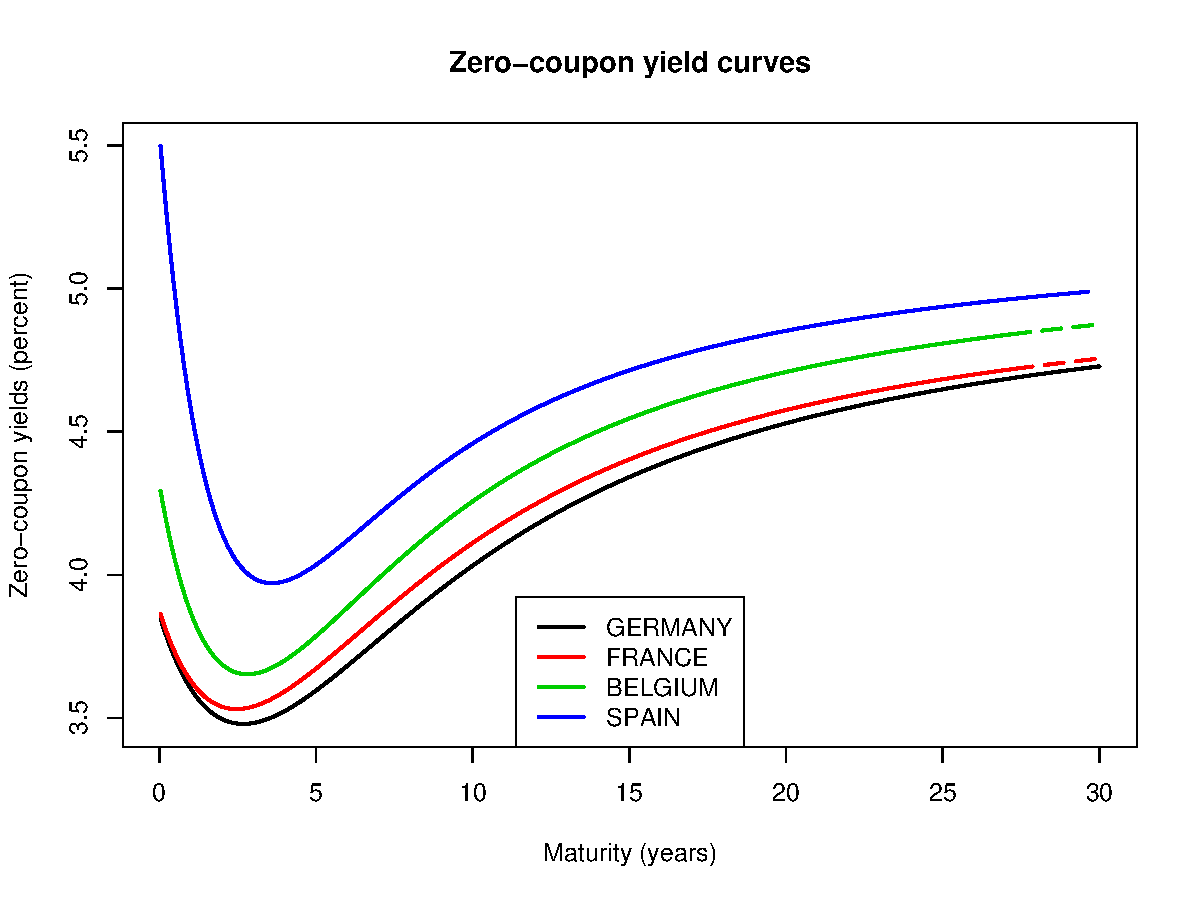
\includegraphics[width=0.7\textwidth]{fig_eurospotcurves}
\end{figure}


\subsection{Spline-based methods}

In this section, we to demonstrate how to estimate the term structure of interest rates with the \cite{McCulloch1975} cubic splines approach applied to French governement bonds.

\begin{Schunk}
\begin{Sinput}
R> y <- splines_estim(c("FRANCE"), govbonds, c(0, 30))
R> y
\end{Sinput}
\begin{Soutput}
---------------------------------------------------
Parameters for Cubic splines estimation:

[1] "FRANCE:"
      alpha 1       alpha 2       alpha 3       alpha 4       alpha 5 
 0.0136620572 -0.0018022601 -0.0003772906  0.0001867318  0.0010633259 
      alpha 6       alpha 7 
 0.0014693772 -0.0408879155 
\end{Soutput}
\end{Schunk}

The summary method shows details from the OLS estimation of the parameters and the goodness of fit measures.

\begin{Schunk}
\begin{Sinput}
R> summary(y)
\end{Sinput}
\begin{Soutput}
---------------------------------------------------
Goodness of fit:
---------------------------------------------------

                   FRANCE
RMSE-Prices  0.1819767236
AABSE-Prices 0.0820766103
RMSE-Yields  0.0005212926
AABSE-Yields 0.0002514331

---------------------------------------------------
Summary statistics for the fitted models:
---------------------------------------------------

$FRANCE

Call:
lm(formula = -Y[[k]] ~ X[[k]] - 1)

Residuals:
      Min        1Q    Median        3Q       Max 
-0.663324 -0.030923 -0.007992  0.041845  0.908719 

Coefficients:
          Estimate Std. Error t value Pr(>|t|)    
alpha 1  0.0136621  0.0072072   1.896    0.066 .  
alpha 2 -0.0018023  0.0020768  -0.868    0.391    
alpha 3 -0.0003773  0.0008139  -0.464    0.646    
alpha 4  0.0001867  0.0002862   0.652    0.518    
alpha 5  0.0010633  0.0001208   8.804 1.66e-10 ***
alpha 6  0.0014694  0.0002102   6.989 3.39e-08 ***
alpha 7 -0.0408879  0.0032007 -12.774 6.14e-15 ***
---
Signif. codes:  0 '***' 0.001 '**' 0.01 '*' 0.05 '.' 0.1 ' ' 1 

Residual standard error: 0.1989 on 36 degrees of freedom
Multiple R-squared:     1,	Adjusted R-squared:     1 
F-statistic: 3.211e+05 on 7 and 36 DF,  p-value: < 2.2e-16 
\end{Soutput}
\end{Schunk}

% <<echo=FALSE>>=
% pdf("fig_frenchspotcurve.pdf", width=8, height=6)
% plot(y,errors="none")
% dev.off()
% @

Figure \ref{fig:frenchspotcurve} shows the yield-to-maturities and the estimated zero-coupon yield curve together with the automatically selected knot points.

\begin{figure}[htb]
\centering
\caption{Zero-coupon yield curve for French government bonds estimated with cubic splines}
\label{fig:frenchspotcurve}
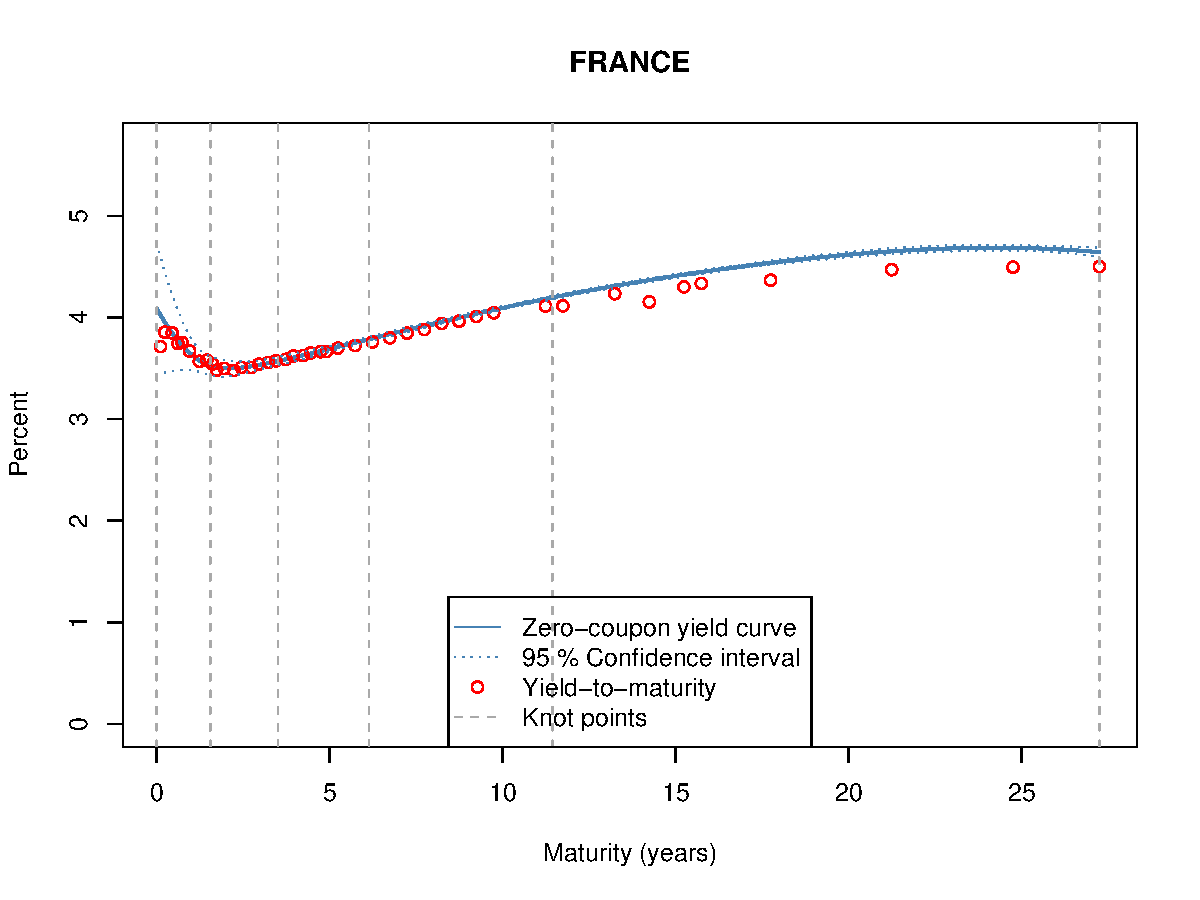
\includegraphics[width=0.8\textwidth]{fig_frenchspotcurve}
\end{figure}

% \begin{figure}[htb]
% \caption{Pricing errors for French government bonds}  
% \begin{center}
% <<fig=TRUE, echo=FALSE>>=
% plot(y,ctype="none", inset=c(0.2, 0.4))
% @
% \end{center}
% \end{figure}

%<<echo=FALSE, fig=FALSE>>=
%pdf("fig_pricingerrors.pdf", width=12, height=8)
%plot(y,ctype="none", inset=c(0.2, 0.4))
%dev.off()
%@

As we can see in Figure \ref{fig:pricingerrors}, there seems to be a misspricing of two bonds. They can be removed and the estimation is redone.

\begin{figure}[htb]
\centering  
\caption{Pricing errors for French government bonds} 
\label{fig:pricingerrors}
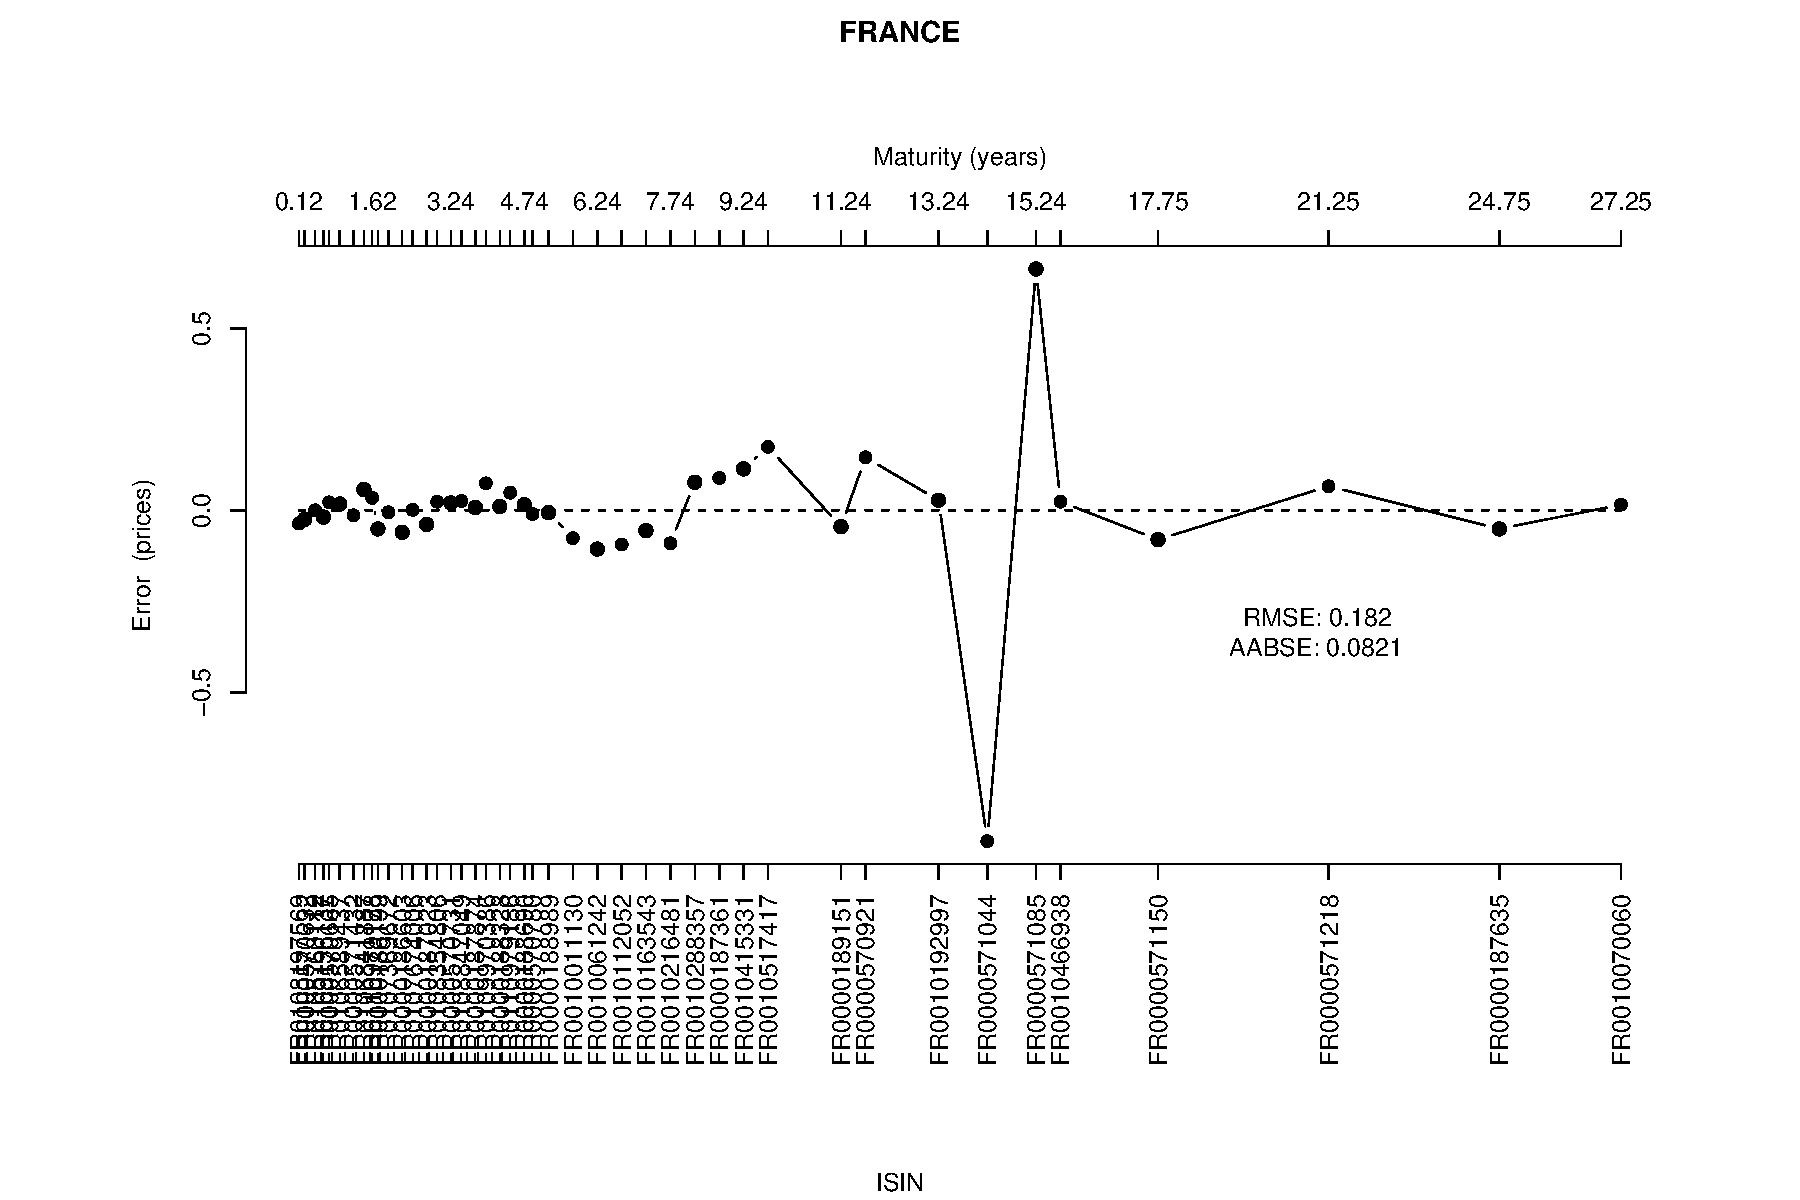
\includegraphics[width=0.8\textwidth]{fig_pricingerrors}
\end{figure}

As expected, the goodness of fit is improved.

\begin{Schunk}
\begin{Sinput}
R> z <- splines_estim(c("FRANCE"), rm_bond(bonddata, c("FR0000571044", 
...    "FR0000571085"), "FRANCE"), c(0, 30))
\end{Sinput}
\end{Schunk}
\begin{Schunk}
\begin{Sinput}
R> summary(z)
\end{Sinput}
\begin{Soutput}
---------------------------------------------------
Goodness of fit:
---------------------------------------------------

                   FRANCE
RMSE-Prices  0.0615589340
AABSE-Prices 0.0515614078
RMSE-Yields  0.0003452360
AABSE-Yields 0.0002025576

---------------------------------------------------
Summary statistics for the fitted models:
---------------------------------------------------

$FRANCE

Call:
lm(formula = -Y[[k]] ~ X[[k]] - 1)

Residuals:
     Min       1Q   Median       3Q      Max 
-0.10516 -0.03516 -0.01789  0.05302  0.14043 

Coefficients:
          Estimate Std. Error t value Pr(>|t|)    
alpha 1  8.886e-03  1.558e-03   5.704 1.89e-06 ***
alpha 2 -9.269e-04  3.869e-04  -2.396   0.0221 *  
alpha 3 -5.500e-04  1.175e-04  -4.682 4.17e-05 ***
alpha 4  9.038e-04  3.307e-05  27.334  < 2e-16 ***
alpha 5  1.526e-03  5.085e-05  30.005  < 2e-16 ***
alpha 6 -3.921e-02  8.287e-04 -47.318  < 2e-16 ***
---
Signif. codes:  0 '***' 0.001 '**' 0.01 '*' 0.05 '.' 0.1 ' ' 1 

Residual standard error: 0.06663 on 35 degrees of freedom
Multiple R-squared:     1,	Adjusted R-squared:     1 
F-statistic: 2.856e+06 on 6 and 35 DF,  p-value: < 2.2e-16 
\end{Soutput}
\end{Schunk}





